\en{Let $ABC$ be a triangle where $\angle BAC = 90^{\circ}$, with circumcenter $O$ and incenter $I$. The angle bisector of $\angle BAC$ intersects the circumcircle of $ABC$ in $A$ and $P$. Let $Q$ be the projection of $P$ onto $AB$, and $R$ be the projection of $I$ onto $PQ$. Prove that $RO$ bisects $CI$.

\bigskip 

\textbf{Solution (Raphael):} Because $O$ is the midpoint of $\overline{BC}$, it suffices to show that $RO$ is parallel to $BI$, as the result follows by simply looking at a homothety centered at $C$.\\
So first of all by looking at the problem we instantly recognise the point P as the circumcenter of $BIC$, as  this is a well know configuration. So from this we get  $|PB| = |PI|$ and $\angle BOP = 90^{\circ}$. Next up we find $AQ$ to be parallel to $IR$, as they both are perpendicular to $PQ$. From this we get $\angle BIR = \angle IBA = \angle IBC$. We now have two same angles at $B$ and $I$ and also $|PB| = |PI|$. This gives us motivation to look at perpendicular bisector of $\overline{BI}$, as it goes through $P$ and $X:= RI \cap BC$. If we can show that $ROX$ is also isosceles, then it'll instantly follow that $\angle BOR = \angle OBI$, which then will give us $RO$ parallel to $BI$ as wanted. So now for the fun stuff; more angle chasing.\\
We easily calculate $\angle APQ = \angle OPB = 45^\circ$. From this we get that $\angle BPQ = \angle OPI$ and thereby that the angle bisector of $\angle IPB$ and $\angle OPR$ coincide. And as the angle bisector of $\angle IPB$ is equal to the perpendicular bisector of $BI$, we have $\angle XPR = \angle OPR$. Finally using the cyclic quadrilateral $OPRX$ we have $\angle ORX = \angle OPX = \angle XPR = \angle XOR$, which finishes the proof as explained before.
}
%RO RO RO your boat, gently down the PX
\de{}



\begin{center}
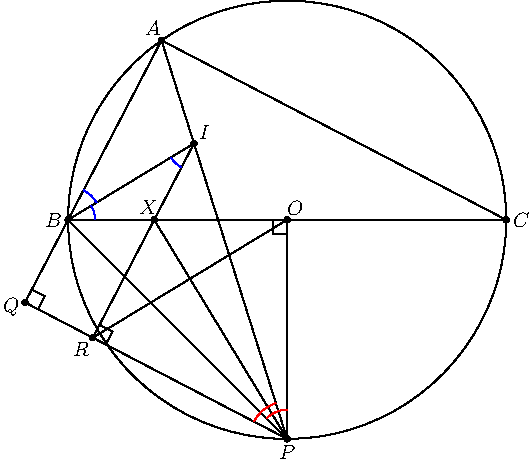
\includegraphics[scale=1]{2021/Selektion/muesterlosung/solutions/s1_fig.pdf}
\end{center}

\textbf{Marking Scheme (additive):}


\begin{itemize}
\item 1P: note that $BPI$ is isosceles or that $\angle BOP = 90^\circ$ or equivalent (WUM)
\item 2P: proof that it suffices to show $BI$ parallel to $RO$
\item 2P: show that the angle bisector of $\angle RPO$, the angle bisector of $\angle BPI$ and the perpendicular bisector of $\overline{BI}$ coincide.
\item 1P: $\angle BOR = \angle OBI $
\item 1P: finish the proof
\end{itemize}
$ $
\\
\textbf{alternative Solution e.g. Emily/Ricardo}\\
Let $S$ be the intersection of $IC$ und $OR$
\begin{itemize}
\item 1P: note that $BPI$ is isosceles or that $\angle BOP = 90^\circ$ or equivalent (WUM)
\item 2P: note $IPC$ isosceles and say that it suffices to show $\angle ISP = 90^\circ$
\item 3P: proof that $PRIS$ is a cyclic quadrilateral
\item 1P: finish the proof
\end{itemize}
